% =============================================================================
% results.tex — Results section (draft v0.3, 2026-09-03)
% Numbers from results_v2/{scenario}/*.csv. All values to be re-checked
% against CSVs before submission; near-term baseline, mature-medium sensitivity.
% =============================================================================

\section{Results}
\label{sec:results}

\subsection{Baseline facility locations and economics}

Without carbon policy, the optimal network serves the two
highest-value demand segments in full and nothing else (Table~\ref{tab:s0};
Fig.~\ref{fig:baseline}). The equilibrium
quantity is 2.30~Mt of biochar per year: the H segment
(\$800/t, 0.80~Mt) and M segment (\$500/t, 1.50~Mt) are fully served, while the
L segment (\$250/t, 2.5~Mt) remains unserved because the marginal cost of
producing and delivering an additional tonne of biochar exceeds \$250/t. The
system surplus is \$708~M/yr in the near-term scenario and \$736~M/yr under
mature-market supply; wet biomass consumption reaches 6.9~Mt/yr (77\% of the
near-term potential). Corn stover is the dominant feedstock (5.9~Mt wet,
fully utilized), supplemented by soybean straw and logging residues. The
optimal facility layout concentrates plants
in the central and southern corn belt, over the feedstock-availability surface
that drives it (Fig.~\ref{fig:baseline}).

\begin{figure}[htbp]
\centering

\includegraphics[width=\textwidth]{figures/fig2_baseline.png}
\caption{\small Baseline network and market clearing (near-term, no policy).
(I) Optimal facility locations over the feedstock-availability surface
(counties shaded by total wet-biomass availability; circles: T1 dehydration,
diamonds: T2 pyrolysis at 300$^\circ$C; marker size proportional to installed
scale tier); plants concentrate in the central and southern corn belt,
co-locating drying and pyrolysis with feedstock so that wet haulage stays
short. (II) Revenue and cost decomposition, leaving a net surplus of
\$708~M/yr. (III) Step demand curve and equilibrium: the marginal supply cost
crosses demand inside the \$500/t M segment, so the H and M segments are fully
served (0.80 and 1.50~Mt) while the \$250/t L segment and the \$30/t sink
remain unserved, the demand-constrained regime that policy must overcome.
Breakpoints at 0.8, 2.3, and 4.8~Mt are marked on the quantity axis; at the
boundary the bid of the marginal served segment (\$500/t at 2.3~Mt) applies.}
\label{fig:baseline}
\end{figure}

\begin{table}[htbp]
\centering
\caption{\small Baseline (S0) system summary, pooled-biochar model (v2); the
quality-differentiated model (v2b) is reported separately in
Table~\ref{tab:v2b}.}
\label{tab:s0}
\begin{tabular}{lcc}
\toprule
 & near-term & mature-market medium\\
\midrule
System surplus (M\$/yr) & 708.3 & 735.7\\
Biochar (Mt/yr) & 2.30 & 2.30\\
\ \ H / M / L served (Mt) & 0.80 / 1.50 / 0 & 0.80 / 1.50 / 0\\
Wet biomass (Mt/yr) & 6.91 & 6.60\\
Net GHG (Mt CO$_2$e/yr) & $-1.60$ & $-1.65$\\
Facilities (T1 / T2-300 / T2-500) & 78 / 38 / 0 & 29 / 18 / 0\\
\bottomrule
\end{tabular}
\end{table}

\FloatBarrier

\subsection{Environmental performance}

The direct atmospheric flux $N(x)=E^{+}(x)-S(x)$ is $-1.60$~Mt CO$_2$e/yr
(process $+979$~kt, transport $+24$~kt, carbon removal $2{,}598$~kt) in
near-term and $-1.65$~Mt (process $+967$~kt, transport $+16$~kt, removal
$2{,}631$~kt) under mature-market supply; it excludes
the decomposition baseline $B(x)\approx 1.35$--$1.65$~t CO$_2$e/t dry, which
enters only the Paradigm~A credit calculation (Section 2.3). Process emissions
dominate the gross flux because drying and pyrolysis are energy-intensive per
delivered tonne, while the sequestration term scales directly with biochar
output; the system is therefore net-negative in both scenarios without any
policy intervention, and its environmental profile is a co-product of the
economic equilibrium rather than a separate objective.

\subsection{Value of biochar and biomass: market-clearing inherent values}

The duals of the node mass balances in the fixed-layout LP
(Fig.~\ref{fig:iv}) reveal the spatial
inherent values of biochar and biomass. In the near-term scenario the inherent
value of biochar ranges \$305--345/t (mean \$324/t), i.e., the marginal value of
an additional tonne of biochar available at a county equals its marginal
production, delivery, and capacity-scarcity cost at the fixed baseline
layout; under mature-market supply this falls to \$260--288/t
(mean \$275/t) because abundant low-cost feedstocks (miscanthus, energy crops)
shrink the scarcity rent. Wet biomass inherent values are far below farmgate
prices (\$0--77/t, mean \$9/t in near-term, Fig.~\ref{fig:iv}), confirming
that the system is
demand-constrained: additional biomass supply is nearly worthless without
additional biochar demand. Following the market-clearing paradigm, these duals
are interpreted as equilibrium prices under a coordinating entity; they are
marginal values conditional on the baseline facility layout, not prices
from a decentralized Nash market (Section~\ref{sec:limitations}). This
demand-constrained structure is exactly the regime in which a linear carbon tax
fails to move the optimum (cf.~\cite{benjaafar2013}).

\begin{figure}[htbp]
\centering

\includegraphics[width=\textwidth]{figures/fig3_inherent_values.png}
\caption{\small Spatial inherent values (duals of the node mass balances;
near-term). (I) Biochar inherent value, \$305--345/t: the marginal value of an
additional biochar tonne at a county. (II) Wet corn stover inherent value,
\$39--77/t, the most valuable biomass series; other wet feedstocks carry
near-zero values (mean \$9/t), confirming the demand-constrained regime in
which marginal biomass supply is nearly worthless without additional biochar
demand. (III) County-level feedstock availability for the nine of 13
feedstocks with nonzero near-term supply (counties sorted by total
availability, feedstocks by abundance; miscanthus, switchgrass, poplar, and
willow have zero near-term supply and are omitted): corn stover dominates the
supply
surface, which is why the optimal network concentrates in the corn belt.}
\label{fig:iv}
\end{figure}

\FloatBarrier

\subsection{Paradigm A: baseline-and-credit}
\label{sec:policyA}

Credits that scale with throughput transform the system (Fig.~\ref{fig:policy}).
At $p_c=\$25$/tCO$_2$e the L segment activates under the calibrated step
demand (0.42~Mt served) and production
rises to 2.72~Mt; at $p_c=\$200$/tCO$_2$e the system saturates its feedstock
potential (2.85~Mt, i.e., essentially 100\% of near-term biomass) and surplus
reaches \$3.36~B/yr. In the
mature-market scenario the response is far larger: 4.79~Mt at $p_c=\$25$ and
$\approx$4.80~Mt at $p_c\ge\$50$, with the L segment fully served from
$p_c=\$25$ and production then pinned at the feedstock ceiling; surplus
reaches \$5.87~B/yr at $p_c=\$200$.
All sweep points solve at a 0.5\% gap target with 600~s time limits (the
$p_c=25/50$ points re-solved with 1{,}800~s limits, improving the
incumbents); reported
gaps are 0.95--1.9\% (near-term) and 0.5--3.2\% (mature-market, SI
Table~S3), and TIME\_LIMIT points are feasible incumbents rather than proven
optima, so their production and surplus figures are lower bounds on
the true policy response. A dedicated re-solve of the mature
$p_c=\$100$ point at a 0.1\% gap target (3{,}600~s, archived as
\texttt{policy\_A\_recert2\_v2.csv}) raised its 500$^\circ$C share from
1.75 to 2.81~Mt at a 1.9\% gap, matching the $p_c=\$150$--\$200 points
(2.81~Mt at 1.0--1.7\% gaps).
Whether credits change the system's technology mix is decided by
which resource binds, not by the credit price alone (Fig.~\ref{fig:creditbasis};
Proposition~\ref{prop:regime} formalizes the crossover prices in the
demand-bound and supply-bound regimes).
In the feedstock-scarce near-term scenario the 300$^\circ$C chain remains
optimal for the bulk (L) segment up to $p_c\approx\$239$/t, because its
yield advantage (0.352 versus 0.278~t/t, feedstock averages) outweighs the modest credit-rate premium
of 500$^\circ$C biochar ($\approx$0.077~tCC/t dry); the binding resource is dry
feedstock, so per-dry-tonne margins rule. In the feedstock-abundant
mature-market scenario the binding resource is biochar demand, and
500$^\circ$C's lower yield multiplies credit revenue per tonne of biochar
served: 500$^\circ$C overtakes 300$^\circ$C at $p_c\approx\$61$/t for every
demand segment, and the sweep routes $\approx$2.8~Mt of the 4.8~Mt through
500$^\circ$C at $p_c=\$100$--\$200. Baseline-and-credit therefore scales the system
in both regimes, but induces a quality upgrade only where feedstock is
abundant, a policy--resource interaction that a single-regime analysis
cannot reveal.
These credits are LCFS-style baseline-and-credit, granted to every
feedstock--temperature pair without an eligibility gate; the VM0044 H/C
gate is applied only in Paradigm~C2 (Section~\ref{sec:policyC}), so Paradigms~A
and C differ in credit basis as well as eligibility
(Fig.~\ref{fig:creditbasis}). The direct atmospheric flux $N(x)=E^{+}(x)-S(x)$
deepens from $-1.60$ to $-1.96$~Mt CO$_2$e/yr as credit prices rise, i.e., net
removal grows with mobilization.

\subsection{Paradigm B: cap-and-trade and the shadow carbon price}

The gross-emission cap sweep traces the system's marginal abatement cost curve
(Fig.~\ref{fig:policy}). Tightening the cap from the baseline 1{,}003~kt to
501~kt reduces surplus from \$708~M to \$451~M/yr and biochar from 2.30 to
1.19~Mt (mature-market: 983$\rightarrow$492~kt, \$736$\rightarrow$\$458~M).
The finite-difference marginal abatement cost is
$\approx$ \$351--391/t CO$_2$e over the first binding intervals and rises to
$\approx$ \$599/t as the cap tightens (mature-market $\approx$ \$468--484
$\rightarrow$ \$603/t), above both 2024--2025 EU ETS allowance prices
(\texteuro 50--90/t, $\approx$\$55--100/t) and the voluntary removal-credit
band (\$100--250/t).
The cap's vertex dual reproduces these values to numerical tolerance: with
Gurobi's sign
convention the reported dual is the negative of the marginal value, i.e.,
$-\$374$/t at the first binding cap (near-term), inside the
\$351--391/t finite-difference band of the first binding intervals, validating the
shadow-price interpretation. Gross emissions are
intrinsic to drying and pyrolysis, so abating them means forgoing biochar
sales, whereas carbon removal is a co-benefit of production; pricing
gross emissions is therefore an expensive lever for this system. The net-flux cap
experiment completes the picture: for $\mathrm{CAP}^{\mathrm{net}}\in[-1{,}000, +1{,}000]$~kt the
constraint $E^{+}(x)-S(x)\le\mathrm{CAP}^{\mathrm{net}}$
does not bind ($\pi=0$) and surplus stays at \$708~M/yr, while a cap of
$-2{,}000$~kt is infeasible under the incumbent dispatch. Every tested cap is
looser than the baseline flux of $-1{,}595$~kt, so this experiment only
establishes that \emph{loose} net caps provide no incentive. A frontier sweep
that tightens the cap below the baseline flux shows where the constraint first
binds and how the system responds (SI Fig.~S2): from $-1{,}600$ to
$-1{,}800$~kt the system deepens its net flux by expanding production into the
unprofitable L segment (2.30$\rightarrow$2.61~Mt, all 300$^\circ$C) at a
finite-difference marginal cost of $\approx$\$110/tCO$_2$e; below
$-1{,}900$~kt further deepening requires converting production to 500$^\circ$C
pyrolysis (0.13$\rightarrow$1.12~Mt over $-1{,}900$ to $-2{,}200$~kt) at
$\approx$\$150--330/tCO$_2$e (finite-difference estimates between
TIME\_LIMIT incumbents), and the minimum feasible net flux is
$-2{,}602$~kt (all-500$^\circ$C, 2.26~Mt, solved to optimality). A net cap is
therefore not blind to negative emissions: it binds once tightened below the
system's own flux, first as an expansion mandate and then as a durability
mandate, with a shadow cost comparable to gross-emission abatement.

\subsection{Paradigm C: tiered tax, VM0044 eligibility, and allocation}
\label{sec:policyC}

The tiered tax (C1) reduces surplus (708 to 653~M\$/yr at rates 25/50/100) but
does not alter the fixed-facility dispatch, consistent with the
demand-constrained regime (Proposition~\ref{prop:taxinv} establishes that a
linear tax cannot change the dispatch when demand is marginally binding).
To rule out the possibility that this null response
is an artifact of the fixed layout, we re-solve C1 as a free-facility MIP
(C1-free): the optimizer finds a layout equivalent to the baseline within the
MIP gap at every rate set tested (Table~\ref{tab:c1free}; 75--80 T1 and
38--40 T2 units versus 78 and 38 at baseline, with gross emissions within
1\% of the baseline dispatch). The free-facility surplus (653.3~M\$/yr)
matches the fixed-layout LP (653.2~M\$/yr) to within the MIP gap, and the same
holds for the steeper (598.3 vs 598.0~M\$/yr) and linear (683.2 vs
683.2~M\$/yr) schedules, confirming that the tax's ineffectiveness
is economic (demand, not emissions, binds) rather than a modeling
artifact. Adding VM0044 removal crediting with free facilities (C2) changes
technology selection directly, because the eligibility gate makes
no 300$^\circ$C biochar credit-eligible: measured 300$^\circ$C chars are
torrefaction-like (H/C $\approx$0.9--1.4), while 500$^\circ$C chars
(H/C $\approx$0.40--0.52) qualify for every feedstock. At $p_c=\$50$ the
near-term system is unchanged (2.30~Mt, all 300$^\circ$C), but the
mature-market system already routes 0.50~Mt to 500$^\circ$C; at
$p_c=\$100$ the incumbent solutions route all production through 500$^\circ$C
in both scenarios: 2.22~Mt
(near-term) and 2.71~Mt (mature-market). At
$p_c=\$200$ production is 2.25~Mt (near-term, surplus \$1{,}141~M/yr, 3.64~Mt
of removal credits) and 4.25~Mt (mature-market, surplus \$1{,}501~M/yr,
7.03~Mt credits), entirely 500$^\circ$C (Fig.~\ref{fig:policy}). Two features
of this result are notable. First, the gate does not subsidize
low-durability biochar: every credited tonne satisfies H/C$\le$0.7, and the
credits purchase durability rather than tonnes. The near-term system's
2.25~Mt falls below the 2.30~Mt H+M demand target because 500$^\circ$C
yields less char per dry tonne, and the mature-market 4.25~Mt remains below
the 4.80~Mt achieved under ungated baseline-and-credit crediting
(Section~\ref{sec:policyA}). Second, full conversion raises gross emissions
(E$^{+}$ grows from 1{,}003 to 1{,}204~kt near-term and from 983 to
2{,}239~kt mature-market) because each delivered biochar tonne now requires
more drying and pyrolysis throughput, exactly the interaction a tiered
emission tax is designed to price. A decomposition experiment isolates the
gate's contribution: with the eligibility gate removed (every char
credit-eligible), the \$200/t near-term system keeps 99\% of production on
300$^\circ$C (2.75 of 2.77~Mt), i.e., the technology conversion is driven by
the eligibility gate rather than by the sequestration credit basis alone (SI
Table~S8). The
allowance-allocation comparison (C3) shows no difference between grandfathering
and benchmarking under fixed facilities: with the layout fixed, gross
emissions are pinned by the demand-constrained dispatch, the allowance budget
is not a binding decision, and the allocation rule merely relabels a fixed
revenue stream. Allocation design therefore matters only when facility
investment is endogenous, an avenue for the multi-period extension. Figure~\ref{fig:policy} consolidates the production,
surplus, and price responses across the three paradigms.

\begin{table}[htbp]
\centering
\caption{\small Tiered tax with free facilities (C1-free): the free-facility MIP
finds a layout equivalent to the baseline within the MIP gap at every rate
set, confirming that the
null tax response is driven by the demand-constrained regime rather than the
fixed-layout approximation (fixed-layout LP surplus in parentheses).}
\label{tab:c1free}
\begin{tabular}{lccccc}
\toprule
 & \multicolumn{2}{c}{near-term} & \multicolumn{2}{c}{mature-market medium}\\
\cmidrule(lr){2-3}\cmidrule(lr){4-5}
rates (r1,r2,r3) & surplus (M\$) & E$^{+}$ (kt) & surplus (M\$) & E$^{+}$ (kt)\\
\midrule
25/50/100 & 653.3 (653.2) & 1{,}003 & 683.1 (681.7) & 985\\
50/100/200 & 598.3 (598.0) & 998 & 629.3 (627.6) & 983\\
25/25/25 (linear) & 683.2 (683.2) & 1{,}002 & 712.9 (711.2) & 983\\
\bottomrule
\end{tabular}
\end{table}

\subsection{Quality-differentiated biochar (v2b)}

Splitting biochar into BC300 and BC500 with the \$800/t CDR premium segment
restricted to BC500 changes the baseline itself: the optimal no-policy network
builds 14~T2-500$^\circ$C facilities and produces 0.80~Mt of BC500, the full
premium segment, alongside 1.50~Mt of BC300
(Fig.~\ref{fig:creditbasis}, Table~\ref{tab:v2b}); the
premium market alone justifies high-temperature pyrolysis. The v2b no-policy
surplus (\$637~M/yr near-term, \$675~M/yr mature-market) is lower than the
pooled-baseline surplus
(\$708~M/yr) because serving the premium segment with BC500 incurs the higher
energy cost and lower yield of 500$^\circ$C pyrolysis; the two models therefore
define different counterfactuals, and cross-model comparisons should focus on
production and technology mix rather than surplus levels. The response to
baseline-and-credit prices follows the two-regime logic of the pooled model.
In the feedstock-scarce near-term scenario, the bulk expansion is served
entirely by BC300 (1.50$\rightarrow$1.84~Mt), and BC500 stays pinned at the
0.80~Mt premium segment, because per-dry-tonne margins keep 300$^\circ$C
optimal for the bulk segment up to $p_c\approx\$239$/t
(Fig.~\ref{fig:creditbasis}). In the
feedstock-abundant mature-market scenario the demand-bound regime takes over:
BC500 rises from 0.80 to 2.77--2.83~Mt at $p_c=\$100$--\$200, roughly 60\% of
the 4.8~Mt total, as 500$^\circ$C's lower yield multiplies credit revenue per
tonne of biochar served above $p_c\approx\$61$/t. Technology selection is
therefore jointly driven by the credit price and the resource regime,
a policy--resource interaction that a pooled-biochar model without quality
differentiation cannot fully reveal, since it also cannot see the
premium-segment floor on BC500.

\begin{figure}[htbp]
\centering

\includegraphics[width=\textwidth]{figures/fig4_policy.png}
\caption{\small Policy response across paradigms A/B/C (near-term). (I) Biochar
production and (II) system surplus against the credit price for
baseline-and-credit (A) and the H/C-gated VM0044-inspired credit (C2), both
shown from their zero-credit point (for C2, the tiered tax alone):
throughput-scaled
crediting expands the system, whereas the gated credit converts it to durable
500$^\circ$C char without expanding tonnage. (III) Marginal abatement cost
traced by the gross-emission cap sweep (finite differences, circles) with the
cap's vertex dual $-\mu_{\mathrm{CAP}}$ (diamonds) and the 2024--2025 RGGI and
EU ETS allowance benchmark bands; the shadow price rises from
$\approx$\$351/tCO$_2$e to
$\approx$\$599/tCO$_2$e, above every observed allowance and voluntary-credit
price. (IV) Technology mix under the H/C gate: the tiered tax leaves the
dispatch
unchanged, but the H/C$\le$0.7 gate excludes every torrefaction-like
300$^\circ$C char and routes all production through 500$^\circ$C pyrolysis as
credit prices rise (all-500$^\circ$C at \$100/t in the incumbent solutions).}
\label{fig:policy}
\end{figure}

\FloatBarrier

\begin{figure}[htbp]
\centering
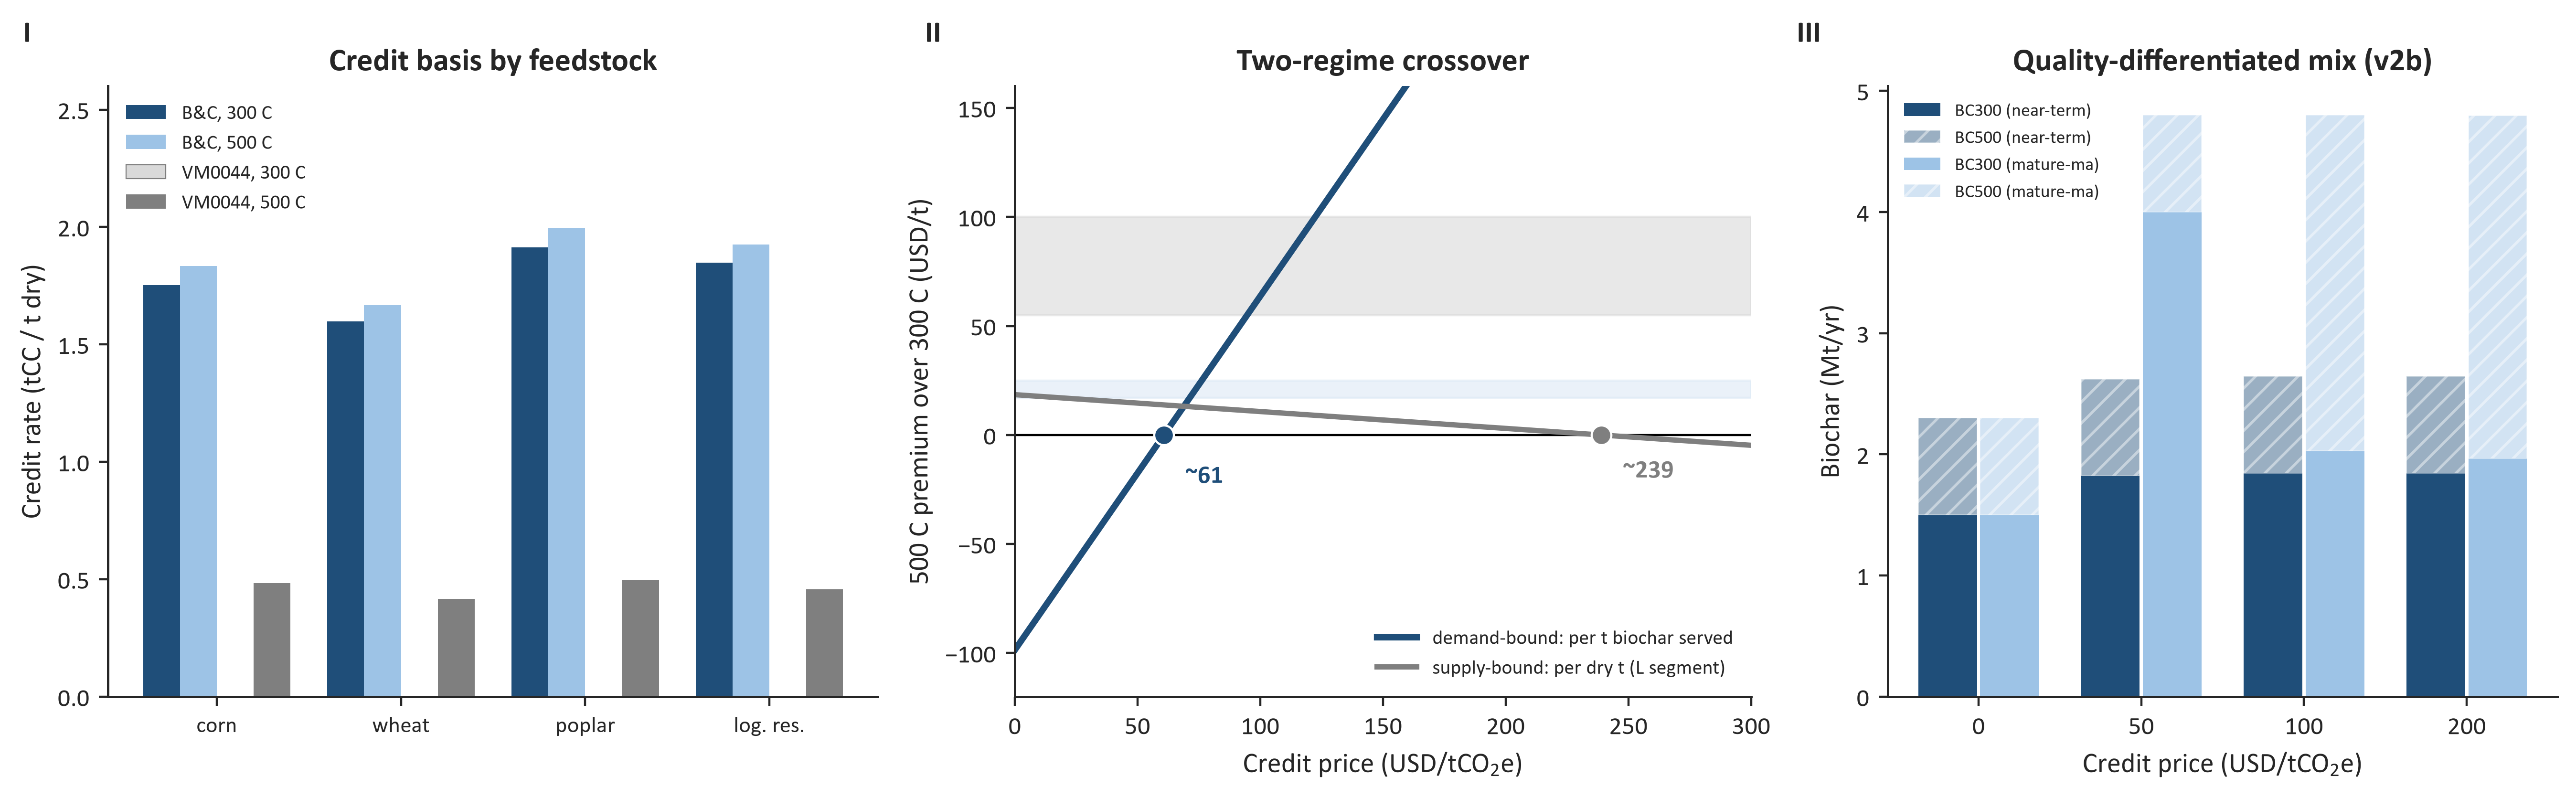
\includegraphics[width=\textwidth]{figures/fig5_credit_basis.png}
\caption{\small Technology choice and credit basis. (I) Carbon credit rates per
tonne dry biomass under the two credit bases (baseline-and-credit, LCFS-style,
$B-E^{+}+S$, versus VM0044, sequestration-based and H/C-gated) for
representative feedstocks and both pyrolysis temperatures; the VM0044 rate of
every torrefaction-like 300$^\circ$C char is zero. (II) The 500$^\circ$C margin
premium over 300$^\circ$C against the credit price in the two resource regimes
(feedstock averages): in the demand-bound regime the binding resource is
biochar demand, so 500$^\circ$C's lower yield multiplies credits per tonne
served and the crossover is at $\approx$\$61/tCO$_2$e for every segment; in the
supply-bound regime per-dry-tonne margins rule and the premium \emph{declines}
with $p_c$ (credits must compensate the yield loss at price $P$), with the bulk
(L) segment
crossing at $\approx$\$239/tCO$_2$e. (III) Quality-differentiated model (v2b):
BC300/BC500 mix under baseline-and-credit in both scenarios; near-term the
premium segment keeps BC500 at 0.80~Mt while expansion runs on BC300, whereas
mature-market BC500 captures 2.77--2.83~Mt.}
\label{fig:creditbasis}
\end{figure}

\begin{table}[htbp]
\centering
\caption{\small Quality-differentiated model (v2b): technology mix under
baseline-and-credit. BC300/BC500 in Mt/yr; surplus in M\$/yr, defined as the
producer objective including credit revenue (policy transfers are decomposed
separately in Table~S7).}
\label{tab:v2b}
\begin{tabular}{lcccccccc}
\toprule
 & \multicolumn{4}{c}{near-term} & \multicolumn{4}{c}{mature-market medium}\\
\cmidrule(lr){2-5}\cmidrule(lr){6-9}
$p_c$ (\$/tCO$_2$e) & BC300 & BC500 & total & surplus & BC300 & BC500 & total & surplus\\
\midrule
0   & 1.50 & 0.80 & 2.30 & 637 & 1.50 & 0.80 & 2.30 & 675\\
50  & 1.82 & 0.80 & 2.62 & 1{,}283 & 4.00 & 0.80 & 4.80 & 1{,}731\\
100 & 1.84 & 0.80 & 2.64 & 1{,}972 & 2.03 & 2.77 & 4.80 & 3{,}092\\
200 & 1.84 & 0.80 & 2.64 & 3{,}350 & 1.97 & 2.83 & 4.80 & 5{,}866\\
\bottomrule
\end{tabular}
\end{table}

\FloatBarrier

\subsection{One-at-a-time sensitivity}
\label{sec:sensitivity}

The baseline solution is far more sensitive to demand-side than to supply-side
parameters (Fig.~\ref{fig:sensitivity}). Demand price $\pm$20\% moves the system
surplus by $\pm$39\% (from \$430~M to \$986~M/yr) while leaving the quantity
at the demand-constrained equilibrium; a 20\% reduction in demand capacity
reduces surplus by 21\% and quantity by 20\%. In contrast, farmgate prices
$\pm$20\% change surplus by only $\pm$9\% and transport costs $\pm$20\% by about
$\pm$1\%; the sink price has no effect because the sink is not activated.

\begin{figure}[htbp]
\centering

\includegraphics[width=\textwidth]{figures/fig6_sensitivity.png}
\caption{\small Sensitivity of the baseline surplus (near-term, fixed facility
layout). (I) One-at-a-time $\pm$20\% perturbations: demand-side parameters
dominate, farmgate and transport are minor, and the feedstock-availability
shock is the only supply-side perturbation of comparable size. (II) Joint
demand sensitivity: system surplus over a grid of demand-price and
demand-capacity multipliers, from \$67~M/yr at $0.6\times$ to \$1{,}406~M/yr at
$1.4\times$; surplus responds smoothly and monotonically to both, with demand
price the larger lever at every capacity level. The baseline $(1.0,1.0)$ cell
reproduces the \$708~M/yr equilibrium.}
\label{fig:sensitivity}
\end{figure}

A
40\% reduction in feedstock availability (a proxy for realistic
field-collection losses) reduces production to 1.48~Mt and surplus by 29\% in
the near-term scenario (from 708.3 to 505.9~M\$/yr), but only by 4\% in the
mature-market scenario: the
system is demand-constrained at the aggregate level, but its preferred
feedstock mix (near-term corn stover) is supply-tight, so availability shocks
matter through the composition of supply even when total demand binds.
These one-at-a-time perturbations hold the baseline facility layout
fixed, so they measure dispatch-level responses; layout-level responses are
captured separately by the free-facility policy sweeps (Paradigms A, C1-free,
and C2). The asymmetry confirms that demand-side instruments (adoption support,
removal crediting) are the effective levers for expanding biochar CDR in
Wisconsin, while feedstock-availability risk concentrates in the corn-stover
supply chain. Two policy-relevant parameter sensitivities complete the
picture. First, the decomposition-baseline assumption (0.9 decay fraction)
enters only Paradigm~A's credit rates: halving it to 0.5 lowers the
\$200/t surplus from \$3.36 to \$2.33~B/yr ($-31$\%) in the near-term and from
\$5.87 to \$3.81~B/yr ($-35$\%) mature-market, while mobilized production stays
near the feedstock potential; the qualitative response and the paradigm
ordering are robust, but the surplus level scales roughly one-for-one with the
baseline assumption and A's magnitude advantage over the gated VM0044 credit
narrows as the decomposition fraction falls. A joint carbon-parameter grid
(decomposition fraction $\{0.5,0.7,0.9\}\times$ permanence multipliers
$\{0.8,1.0,1.2\}$, nine free-facility MIP re-solves at $p_c=\$200$/t, gaps
1.2--1.7\%) shows the two parameters act nearly additively: halving the
decomposition fraction lowers the \$200/t surplus by 31--34\% at every
permanence level, a $\pm$20\% permanence perturbation moves the surplus by
only $\mp$3--5\%, and the near-term technology mix remains essentially
all-300$^\circ$C (at most 0.22~Mt of 500$^\circ$C) in every cell (SI,
carbon-parameter scenarios). Second,
the premium-segment capacity directly sets the scale of 500$^\circ$C
deployment: halving H to 0.4~Mt halves BC500 to 0.40~Mt (total production
1.90~Mt), and enlarging H by 50\% (1.2~Mt) raises BC500 to 1.20~Mt and total
production to 2.52~Mt near-term (2.70~Mt mature); the premium market, not
production cost, is the binding driver of high-temperature pyrolysis.
